%compile with xelatex --shell-escape ContextFreeConstrainedPathFindingInGraph.tex

% v2-acmtog-sample.tex, dated March 7 2012
% This is a sample file for ACM Transactions on Graphics
%
% Compilation using 'acmtog.cls' - version 1.2 (March 2012), Aptara Inc.
% (c) 2010 Association for Computing Machinery (ACM)
%
% Questions/Suggestions/Feedback should be addressed to => "acmtexsupport@aptaracorp.com".
% Users can also go through the FAQs available on the journal's submission webpage.
%
% Steps to compile: latex, bibtex, latex latex
%
% For tracking purposes => this is v1.2 - March 2012
\documentclass{sig-alternate} % V1.2

%\acmVolume{VV}
%\acmNumber{N}
%\acmYear{YYYY}
%\acmMonth{Month}
%\acmArticleNum{XXX}
%\acmdoi{10.1145/XXXXXXX.YYYYYYY}
\usepackage{graphicx}
\usepackage{caption}
\usepackage{subcaption}
\usepackage{gnuplottex}
\usepackage{tikz}
%\usepackage[T2A]{fontenc} 
%\usepackage[utf8]{inputenc}
\usepackage{graphicx}
%\usepackage{indentfirst}
\usepackage{hyperref}
\usepackage{textcomp}

\usepackage{algpseudocode}
\usepackage{algorithm}
\usepackage{algorithmicx}


\begin{document}

\newtheorem{mytheorem}{Theorem}
\newtheorem{lemma}{Lemma}

\algnewcommand\algorithmicswitch{\textbf{switch}}
\algnewcommand\algorithmiccase{\textbf{case}}
\algnewcommand\algorithmicassert{\texttt{assert}}
\algnewcommand\Assert[1]{\State \algorithmicassert(#1)}
% New "environments"
\algdef{SE}[SWITCH]{Switch}{EndSwitch}[1]{\algorithmicswitch\ #1\ \algorithmicdo}{\algorithmicend\ \algorithmicswitch}
\algdef{SE}[CASE]{Case}{EndCase}[1]{\algorithmiccase\ #1}{\algorithmicend\ \algorithmiccase}

\algtext*{EndSwitch}
\algtext*{EndCase}
\algtext*{EndWhile}% Remove "end while" text
\algtext*{EndIf}% Remove "end if" text
\algtext*{EndFor}% Remove "end for" text
\algtext*{EndFunction}% Remove "end function" text


\makeatletter
\def\@copyrightspace{\relax}
\makeatother

\title{Generalized LL parsing for context-free constrained path search problem}

\sloppy

\numberofauthors{2}

\author{
\alignauthor
       Semyon Grigorev\\
       \affaddr{Saint Petersburg State University}\\
       \affaddr{7/9 Universitetskaya nab.}\\
       \affaddr{St. Petersburg, 199034 Russia}\\
       \email{semen.grigorev@jetbrains.com}
\alignauthor
       Anastasiya Ragozina\\
       \affaddr{Saint Petersburg State University}\\
       \affaddr{7/9 Universitetskaya nab.}\\
       \affaddr{St. Petersburg, 199034 Russia}\\
       \email{ragozina.anastasiya@gmail.com}
}

\maketitle

\begin{abstract}
Graph data model and graph data bases are very popular in many 
different areas such as bioinformatics, semantic web, social networks etc. 
One of specific problem on graph DB is a path querying with constrains 
formulated in terms of formal grammars. There is number of solutions, but
building structural representation of query result which practical for 
answer understanding and exploration is still a problem. 
%At the same time it is important to adopt advanced parsing algorithm to give 
In this paper we propose graph parsing technique which allows to build such representation with respect to given grammar query for arbitrary context-free grammar and graph.
Proposed algorithm is based on generalized top-down parsing algorithm which have cubic worst-case time complexity and linear for LL grammars.

\end{abstract}

\section{Introduction}
Graph data model and graph data bases are very popular in many different areas such as bioinformatics, semantic web, social networks etc.
Extraction of paths satisfying specific constraints may be useful for graph structured data investigation and for relations between data items detection.
One of specific problem is a path querying with constrains formulated in terms of formal grammars: formal language constrained path problem~\cite{FLCpathProblem}.

%!!!!!!!!!!!!!!!!!!!!!!!!!!!!!!!!!!!!!!!!!!!!
%Information from different areas such as bioinformatic, semantic web, social networks can be represented in graph model. 
%Moreover, there are data graph data bases. (?) One of the common graph problem is paths extraction from graph. 
%Paths must satisfy specific constrains and the search must use a reasonable time. (?)     
%!!!!!!!!!!!!!!!!!!!!!!!!!!!!!!!!!!!!!!!!!!!!

Classical parsing techniques can be used to solve formal language constrained path problem. 
It means that such technique can be used on more common problem --- ``graph parsing''. 
Graph parsing may be required in graph data base querying, formal verification, string-embedded language processing and another areas where graph structured data. 


The most existing solutions in DB area use such parsing algorithms as CYK or Earley(for example~\cite{ConjCFPathQuery}, ~\cite{GraphQueryWithEarley}). These algorithms have nonlinear time complexity ($O(n^3)$ and $O(n^2)$ respectively), but there are exist such parsing algorithms as GLR and GLL, witch have cubic worst-case complexity and linear for unambiguous grammars.  
Complexity is $O(n^3)$ in worst case and linear for unambiguous grammars, that better than complexity of CYK and Earley which used as base in other solutions (for example~\cite{ConjCFPathQuery}, ~\cite{GraphQueryWithEarley})that better than complexity of CYK and Earley.
This fact allows to demonstrate better performance in some cases, on linear subgraphs and unambiguous grammars, for example. 
Also it is not necessary to transform input grammar to CNF which required for CYK which allows to avoid grammar size increasing.
It is important because real performance of parsing algorithm is sensitive to grammar size.

Despite the fact that there is a set of path querying solutions~\cite{GraphQueryWithEarley, ConjCFPathQuery, !!!}, query result exploration is still a challenge~\cite{hofman2015separabilityForRegQueryDebugging}. 
Simplification of complex query debugging is also a problem.
To solve these problems structural representation of query result can be useful, and classical parsing techniques allow to construct such representation: derivation tree contains full information about parsed sentence structure in terms of specified grammar.

Graph parsing can be also used in dynamically generated strings or string-embedded languages processing. 
Regular approximation for value set of string variable can be represented as graph of related finite automata.
As a next step, for example, in order to check correctness of dynamically generated strings we should to check that all generated strings (all paths from start states to final states) are correct with respect to some context-free grammar.
For example grammar of one of SQL dialects can be used for processing string-embedded SQL.
There are some solutions addressed this problem: GLR-based checker of string-embedded SQL queries~\cite{Alvor1, Alvor2};
relaxed parser of string-embedded languages~\cite{relaxedRNGLR} based on RNGLR parsing algorithm. The latest one allows to construct derivation forest for all correct path in input automata.

In this paper we propose graph parsing technique which allows to construct structural representation of query result with respect to given grammar query.
This structure can be useful for query debugging and exploration, or for other purposes. 
Proposed algorithm is based on generalized top-down parsing algorithm --- GLL~\cite{GLL} --- which have cubic worst-case time complexity and linear for LL grammars.  

\section{Preliminaries}

In this work we are focused on the parsing algorithm, and not on the data representation, and we assume that whole input graph can be located in RAM memory in the optimal for our algorithm way.

We start by introduction of necessary definitions.
\begin{itemize}
  \item Context-free grammar is a quadruple $G=(N, \Sigma, P, S)$, where $N$ is a set of nonterminal symbols, $\Sigma$ is a set of terminal symbols, $S \in N$ is a start nonterminal, and $P$ is a set of productions. 
  \item $\mathcal{L}(G)$ denotes a language specified by grammar $G$, and is a set of terminal strings derived from start nonterminal of $G$: $L(G) = \{\omega | S \Rightarrow_{G}^{*} \omega\}$.
  \item Directed graph is a triple $M = (V,E,L)$, where $V$ is a set of vertices, $L \subseteq \Sigma$ is a set of labels, and a set of edges $E\subseteq V\times L\times V$. 
  We assume that there are no parallel edges with equal labels: for every $e_1=(v_1,l_1,v_2) \in E, e_2=(u_1,l_2,u_2) \in E$ if $v_1 = u_1$ and $v_2 = u_2$ then $l_1 \neq l_2$.
  \item $tag: E \rightarrow L$ is a helper function which allows to get tag of edge. $$tag(e = (v_1,l,v_2), e \in E) = l$$
  \item $\oplus: L^+ \times L^+ \rightarrow L^+$ denotes a tag concatenation operation.
%  \item Path $p$ in graph $M$ is a list of incident edges: 
%  \begin{align*}
%   p &= e_0,e_1,\dots,e_{n-1} \\
%     &= (v_0,l_0,v_1),(v_1,l_1,v_2),\dots,(v_{n-1},l_{n-1},v_n)
%  \end{align*}
%  where $v_i \in V$, $e_i \in E$, $e_i=(v_i,l_i,v_{i+1})$, $l_i \in L$, $|p| = n, n \geq 1$. 
%  \item $P$  is a set of paths $\{p: p \text{ path in } M\}$, where $M$ is a directed graph.
%  \item $\Omega: P \rightarrow L^+$ is a helper function which constructs a string produced by the given path. For every $p \in P$
  \item $\Omega$ is a helper function which constructs a string produced by the given path. For every $p \text{ path in } M$
  \begin{align*}
  & \Omega(p = e_{0},e_{1},\dots,e_{n-1}) = \\
  & tag (e_{0}) \oplus \dots \oplus tag (e_{n-1}).
  \end{align*}
\end{itemize}

Using these definitions, we state the context-free language constrained path querying as, given a query in form of grammar $G$, to construct the set of paths $$Q(M,G)=\{p|p \text{ is path in } M, \Omega(p) \in \mathcal{L}(G)\}.$$

Note that, in some cases, $Q(M,G)$ can be an infinite set, and hence it cannot be represented explicitly. 
In order to solve this problem, in this paper, we construct compact data structure representation which stores all elements of $Q(M,G)$ in finite amount of space and allows to extract any of them.

\subsection{Generalized LL Parsing Algorithm}\label{BasicGLL}

One of widely used classes of parsing algorithms is a LL(k)~\cite{Grune}---top-down algorithms which read input from left to right, build leftmost derivation, and use $k$ symbols for lookahead.
LL(k) parser may be implemented as deterministic pushdown automaton (DPDA).
On the other hand LL(k) parser may be implemented in recursive-descent manner: each rule transforms to function which can call functions for other rules in order specified by right hand side of corresponded rule.
In this case stack of DPDA are replaced with functions call stack.

Classical LL algorithm operates with a pointer to input (position $i$) and with a grammar slot---pointer to grammar in form $N \rightarrow \alpha \cdot x \beta $.
Parsing may be described as a transition of these pointers from the initial position ($i = 0$, $S \rightarrow \cdot \beta $, where $S$ is start nonterminal) to the final ($i = input.Length$, $s \rightarrow \beta \cdot$).
At every step, there are four possible cases in processing of these pointers. 

\begin{enumerate}
\item $N \rightarrow \alpha \cdot x \beta $, when $x$ is a terminal and $x = input[i]$. In this case both pointers should be moved to the right ($i \leftarrow i + 1$, $N \rightarrow \alpha  x \cdot \beta $).
\item $N \rightarrow \alpha \cdot X \beta $, when $X$ is nonterminal. In this case we push return address $N \rightarrow \alpha X \cdot \beta $ to stack and move pointer in grammar to position $X \rightarrow \cdot \gamma$.\label{itm:2}
\item $N \rightarrow \alpha \cdot $. This case means that processing of nonterminal $N$ is finished. We should pop return address from stack and use it as new slot.\label{itm:3}
\item $S \rightarrow \alpha \cdot $, where $S$ is a start nonterminal of grammar. In this case we should report success if $i = input.Length - 1$ or failure otherwise. 
\end{enumerate}

In the second case there can be several slots $X \rightarrow \cdot \gamma$ due to the fact that this algorithm is nondeterministic, so a strategy on how to choose one of them to continue parsing is needed.
In LL(k) algorithm lookahead is used to avoid nondeterminism, but this strategy is still not good enough because there are context-free languages for which deterministic choice is impossible even for infinite lookahead~\cite{LLnonLL}.
On the contrary to LL(k), generalized LL does not choose at all, handling all possible variants by using descriptors mechanism.
Descriptor is a quadruple $(L, s, j, a)$ where $L$ is a grammar slot, $s$ is a stack node, $j$ is a position in the input string, and $a$ is a node of derivation tree.
Each descriptor fully describes one parser state, thus instead of immediate processing of all variants, GLL store all possible branches and process them sequentially late.

The stack in parsing process is used to store return information for the parser---a state to return for continue after finishing current state processing.
%name of function which will be called when current function finishes computation. 
As mentioned before, generalized parsers process all possible derivation branches and parser must store it's own stack for every branch. 
It leads to an infinite stack growth being done naively.  
Tomita-style graph structured stack (GSS)~\cite{Tomita} combines stacks resolving this problem.
Each GSS node contains a pair of position in input and a grammar slot in GLL. 

In order to provide termination and correctness, we should avoid duplication of descriptors, and be able to process GSS nodes in arbitrary order. It is necessary to use the following additional sets for this.
\begin{itemize}
\item $R$---working set which contains descriptors to be processed. Algorithm terminates whenever $R$ is empty.
\item $U$---all created descriptors. Each time when we want to add a new descriptor to $R$, we try to find it in this set first.
This way we process each descriptor only once which guarantee termination of parsing.
\item $P$---popped nodes. Allows to process descriptors (and GSS nodes) in arbitrary order. 
\end{itemize}

%Instead of explicit code generation used in classical algorithm, we use table version of GLL~\cite{TableGLL} in order to simplify adaptation to graph processing.
%As a result, main control function is different from the original one because it should process LL-like table instead of switching between generated parsing functions.
%Control functions of the table based GLL are presented in Algorithm~\ref{mainTblFunctions}.
%All other functions are the same as in the original algorithm and their descriptions can be found in the original article~\cite{scott2010gll}.

%\begin{algorithm}[ht]
%\begin{algorithmic}[1]
%\caption{Control functions of table version of GLL}
%\label{mainTblFunctions}
%\Function{dispatcher}{ \ }
%  \If{$R.Count \neq 0$}  
%      \State{$(L,v,i,cN) \gets R.Get()$}
%      \State{$cR \gets dummy$}
%      \State{$dispatch \gets false$}
%  \Else
%      \State{$stop \gets true$}
%  \EndIf
%\EndFunction
%
%\Function{processing}{ \ }
%  \State{$dispatch \gets true$}
%  \Switch{$L$}
%  \Case{$(X \rightarrow \alpha \cdot x \beta)$ where $x = input[i + 1])$}
%       \If{$cN = dummyAST$} 
%          \State{$cN \gets \Call{getNodeT}{i}$} 
%       \Else 
%          \State{$cR \gets \Call{getNodeT}{i}$}
%       \EndIf
%       \State{$i \gets i + 1$}
%       \State{$L \gets (X \rightarrow \alpha x \cdot \beta)$}
%       \If{$cR \neq dummy$}
%          \State{$cN \gets \Call{getNodeP}{L, cN, cR}$} 
%       \EndIf
%       \State{$dispatch \gets false$}        
%  \EndCase
%  \Case{$(X \rightarrow \alpha \cdot x \beta)$ where $x$ is nonterminal}
%       \State{$v \gets$ \Call{create}{$(X \rightarrow \alpha x \cdot \beta), v, i, cN$}}
%       \State{$slots \gets pTable[x][input[i]]$}
%       \ForAll{$L \in slots$}
%          \State{\Call{add}{$L,v,i,dummy$}} 
%       \EndFor
%  \EndCase
%  \Case{$(X \rightarrow \alpha \cdot )$}
%       \State{\Call{pop}{v,i,cN}} 
%  \EndCase
%  \Case{$(S \rightarrow \alpha \cdot )$ when $S$ is start nonterminal}
%       \State{final result processing and error notification} 
%  \EndCase
%  \EndSwitch
%\EndFunction
%
%\Function{control}{}
%  \While{not $stop$}  
%      \If{$dispatch$}
%        \State{\Call{dispatcher}{ \ }}
%      \Else
%         \State{\Call{processing}{ \ }}
%      \EndIf
%  \EndWhile
%\EndFunction
%
%\end{algorithmic}
%\end{algorithm}

There can be more than one derivation tree of a string with relation to ambiguous grammar.
Generalized LL build all such trees and compact them in a special data structure Shared Packed Parse Forest~\cite{SPPF}, which will be described in the following section.

\subsection{Shared Packed Parse Forest}

Binarized Shared Packed Parse Forest (SPPF)~\cite{brnglr} compresses derivation trees optimally reusing common nodes and subtrees.
Version of GLL which uses this structure for parsing forest representation achieves worst-case cubic space complexity~\cite{gllParsingTree}.

Binarized SPPF can be represented as a graph in which each node has one of four types described below.
Let $i$ and $j$ be the start and the end positions of substring, and let us call a tuple $(i,j)$ an \textit{extension} of node.

\begin{itemize}
    \item \textbf{Terminal node} with label $(i, T, j)$.
    \item \textbf{Nonterminal node} with label $(i, N, j)$. 
    This node denotes that there is at least one derivation for substring $\alpha=\omega[i..j-1]$ such that $N \Rightarrow^*_G \alpha, \alpha = \omega[i..j-1] $.
    All derivation trees for the given substring and nonterminal can be extracted from SPPF by left-to-right top-down graph traversal started from respective node.     
    \item \textbf{Intermediate node}: a special kind of node used for binarization of SPPF. These nodes are labeled with $(i,t,j)$, where $t$ is a grammar slot.
    \item \textbf{Packed node} with label $(N \rightarrow \alpha \cdot \beta, k)$. 
    Subgraph with ``root'' in such node is one variant of derivation from nonterminal $N$ in case when the parent is a nonterminal node labeled with $(<\mkern-9mu | \mkern-9mu> (i, N, j))$.

\end{itemize}

Example of SPPF presented in figure~\ref{SPPF}. We remove redundant intermediate and packed nodes from the SPPF to simplify it and to decrease the size of structure.

\section{Motivating Example}\label{motivExample}

Suppose that you are student in a School of Magic.
It is your first day in the School, so navigation in the building is a problem for you.
Fortunately, you have a map of the building (fig.~\ref{input}) and an additional knowledge about building construction:
\begin{itemize}
  \item there are towers in the school (nodes of the graph in your map);
  \item all floors of some towers connected by directed galleries (edges in your map);
  \item each gallery has a ``magic'' property: start floor is aways one more (edge label is 'b') or one less (edge label is 'b') then end floor. 
\end{itemize}

\begin{figure}[h]
    \begin{center}
        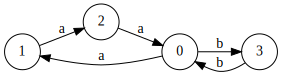
\includegraphics[width=6cm]{dot/input.pdf}
        \caption{The map of School (input graph $M$)}
        \label{input}        
    \end{center}
\end{figure}


You want to find a path from your current position to the same floor in another tower. 
Map with all such paths can help you.
But orienteering is not your forte, so it would be great if the structure of the paths were as simple as possible and all paths will have checkpoints to control your rout.

It is evident that the simplest structure of required paths is $\{ab, aabb, aaabbb, \dots\}$.
In terms of our definitions you have a graph $M=(\{0;1;2;3\},E,\{a;b\})$ (figure~\ref{input}), and you want to find all paths $p$, such that $\Omega(p) \in \{ab; aabb; aaabbb; \dots\}$ or $\Omega(p) \in a^n b^n$ where $n \geq 1$.


Unfortunately, language $\mathcal{L} = \{a^n b^n; n \geq 1\}$ is not regular which restricts the set of tools you can use. 
Another problem is the infinite size of solution, but you want to get a finite map.  
Moreover, you want to know a structure of paths with checkpoints added.

We are not aware of any existing tools which can help to solve this problem and we create a new one.
Let us to show how to get the map which help to orient in this strange School.

Fortunately, the language $\mathcal{L} = \{a^n b^n; n \geq 1\}$ is a context-free language and can be specified with context-free grammar. 
The fact that one language can be described with more than one grammar allows to add checkpoints: additional nonterminals can mark required parts of a sentence.
In our case, a desired checkpoint can be in the middle of the path.
As a result, required language can be specified by the grammar $G_1$ presented in figure~\ref{grammarG}, where $N = \{s; \text{\textit{Middle}}\}$, $\Sigma = \{a; b\}$, and $S$ is a start nonterminal.

\begin{figure}[h]
   \begin{center}
   \[
\begin{array}{rl}
   0:& S \rightarrow a \ S \ b \\
   1:& S \rightarrow Middle \\
   2:& Middle \rightarrow a \ b
\end{array}
\]

   \caption{Grammar $G_1$ for language $L=\{a^n b^n; n \geq 1\}$ with additional marker for a middle of a path}
   \label{grammarG}        
   \end{center}
\end{figure}

In the next section we present a map construction algorithm,  which solves such problems.

\section{Graph Parsing Algorithm}

We propose a context-free language constrained path problem solution which allows to create finite representation of parse forest which contains trees for all satisfied paths in graph.
Finite representation of result set with structure related to specified grammar may be useful not only for results understanding and processing but also for query debugging especially for complex queries. 

Our solution is based on generalized LL (GLL)~\cite{scott2010gll, FastPracticalGLL} parsing algorithm which allows to process arbitrary (including left-recursive and ambiguous) context-free grammars with worst-case cubic time complexity and linear for LL grammars. 

\subsection{Generalized LL Parsing Algorithm}

In classical LL algorithm we have pointer in input and pointer in grammar of form $n \rightarrow \alpha \cdot x \beta $ --- grammar slot.
Parsing may be described as related movement this pointers from initial position. Thus in each step we have two pointers and some possible cases to process them. 

\begin{enumerate}
\item $n \rightarrow \alpha \cdot x \beta $ when $x$ is a terminal and $x = input[i]$ 
\item $n \rightarrow \alpha \cdot x \beta $ when $x$ is nonterminal
\item $n \rightarrow \alpha \cdot $
\item $s \rightarrow \alpha \cdot $
\end{enumerate}

In case (2) we can use $FIRST$ set to choose single variant. 
But sometimes it is not possible to select only one path to continue parsing and it does not allow to use LL parsing algorithm.
Generalized LL algorithm handle all possible paths in this case. 
Instead of immediate processing of all variants GLL uses descriptors mechanism to store all possible branches and process them sequentially. 
Descriptor is a quadriple $(L, s, j, a)$ where $L$ is a grammar slot, $s$ is a stack node, $j$ is a position in the input, and $a$ is a node of derivation tree. 

Stack in parsing process is used to store return information for the parser --- a name of function which would be called when current function will finish computing. 
As previously mentioned, generalized parsers process all possible derivation branches and for every branch parser must store it's own stack. It leads to infinite stack grow.  
Tomita-style graph structured stack (GSS)~\cite{Tomita} allows to combine stacks to solve this problem.
In GLL each GSS node contains a pair of position in input and grammar slot. 

Detailed description of GLL parsing algorithm is available in this article~\cite{GLL}. Pseudocode of stack and tree manipulation functions can be found in Appendix~\ref{GLLCode}.

$R$ ---   
We use table version~\cite{TableGLL} instead of code generation.

\begin{algorithm}[h]
\begin{algorithmic}[1]
\caption{Control functions}
\label{mainFunctions}
\Function{dispatcher}{}
  \If{$R.Count \neq 0$}  
      \State{$(L,v,i,cN) \gets R.Get()$}
      \State{$cR \gets dummy$}
      \State{$dispatch \gets false$}
  \Else
      \State{$stop \gets true$}
  \EndIf
\EndFunction

\Function{processing}{}
  \State{$dispatch \gets true$}
  \Switch{$L$}
  \Case{$(X \rightarrow \alpha \cdot x \beta)$ where $x = input[i + 1])$}
       \If{$cN = dummyAST$} 
          \State{$cN \gets \Call{getNodeT}{i}$} 
       \Else 
          \State{$cR \gets \Call{getNodeT}{i}$}
       \EndIf
       \State{$i \gets i + 1$}
       \State{$L \gets (X \rightarrow \alpha x \cdot \beta)$}
       \If{$cR \neq dummy$}
          \State{$cN \gets \Call{getNodeP}{L, cN, cR}$} 
       \EndIf
       \State{$dispatch \gets false$}        
  \EndCase
  \Case{$(X \rightarrow \alpha \cdot x \beta)$ where $x$ is nonterminal}
       \State{$v \gets$ \Call{create}{$(X \rightarrow \alpha x \cdot \beta), v, i, cN$}}
       \State{$slots \gets pTable[x][input[i]]$}
       \ForAll{$L \in slots$}
          \State{\Call{add}{L,v,i,dummy}} 
       \EndFor
  \EndCase
  \Case{$(X \rightarrow \alpha \cdot )$}
       \State{\Call{pop}{v,i,cN}} 
  \EndCase
  \Case{$(S \rightarrow \alpha \cdot )$ when $S$ is start nonterminal}
       \State{final result processing and error notification} 
  \EndCase
  \EndSwitch
\EndFunction

\Function{control}{}
  \While{not $stop$}  
      \If{$dispatch$}
        \State{\Call{dispatcher}{}}
      \Else
         \State{\Call{processing}{}}
      \EndIf
  \EndWhile
\EndFunction

\end{algorithmic}
\end{algorithm}

There are more than one tree for ambiguous grammar and generalized algorithms builds all derivation trees. Special data structure --- SPPF --- is used to reduce space required for tree storage.


\subsection{Shared packed parse forest}

Shared Packed Parse Forest (SPPF)~\cite{SPPF} is a special data structure for derivation forest compact representation which allow to reuse common nodes and subtrees.
As a result multiple derivation trees, which can be produced in case of ambiguous grammar, can be compressed in one SPPF with optimal reusing of common parts.  
Binarized form of SPPF proposed in~\cite{brnglr} and it allow to achieve worst-case cubic space complexity.
GLL can use SPPF~\cite{gllParsingTree} for results representation achieve cubic space complexity with binarised version.

Let we present an example of SPPF for ambiguous grammar $G_0$ (pic~\ref{grammarG0}).

\begin{figure}[h]
   \begin{center}
\begin{verbatim}
   0: s = eps
   1: s = A s B
   2: s = s s
\end{verbatim}
   \caption{Grammar $G_0$}
   \label{grammarG0}        
   \end{center}
\end{figure}


Let we parse the sentence \verb|"ABABAB"|. 
There are two different leftmost derivations of this sentence in grammar $G_0$, hence SPPF should contains two different trees and it is presented in figure~\ref{sppfSample}: result SPPF(fig. ~\ref{sppf}) and trees for derivation 1(fig.~\ref{tree1}) and derivation 2(fig.~\ref{tree2}) respectively. 
 
\begin{figure*}[ht]
    \begin{center}
    \centering
    \begin{subfigure}[b]{0.3\textwidth}
        \includegraphics[width=\textwidth]{dot/Brackets.pdf}
        \caption{SPPF}
        \label{sppf}        
    \end{subfigure}
    ~
    \begin{subfigure}[b]{0.3\textwidth}
        \includegraphics[width=\textwidth]{dot/Brackets.pdf}
        \caption{Tree for derivation 1}
        \label{tree1}        
    \end{subfigure}
    ~
    \begin{subfigure}[b]{0.3\textwidth}
        \includegraphics[width=\textwidth]{dot/Brackets.pdf}
        \caption{Tree for derivation 2}
        \label{tree2}        
    \end{subfigure}
    \caption{SPPF for sentence \textbf{\texttt{"(1)(2)(3)"}} and grammar $G_0$}
    \label{sppfSample}
    \end{center}                
\end{figure*}

Binarised SPPF can be represented as a graph where each node has one of four types which described below with corresponded graphical notation.

\begin{itemize}
    \item Node with rectangle shape labeled with $(i, T, j)$ is terminal node.     
    \item Node with oval shape labeled with $(i, N, j)$ is nonterminal node. 
    This node denote that there is at least one derivation for substring $\alpha$ from position $i$ to position $j$ in input string $\omega$ such that $N \Rightarrow^*_G \alpha, \alpha = \omega[i..j-1] $.
    All derivation trees for given substring and nonterminal can be extracted from SPPF by left-to-right top-down graph traversal started from respective node. 
    We use filled nonterminal node labeled with $(<\mkern-11mu | \mkern-11mu> (i, N, j))$ for denote that there are more then one derivations from nonterminal $N$ for substring from $i$ to $j$.
    \item Intermediate node with label $(i,t,j)$ where $t$ is a grammar slot. We use dot shape for these nodes and omit label because it is important only for SPPF constriction.
	Subgraph with root in such node is one variant of derivation in case when parent is nonterminal node with label $(<\mkern-9mu | \mkern-9mu> (i, N, j))$.
    \item Node with rectangle shape and label $(N : \gamma \cdot, k)$ is a packed node.
\end{itemize}
One of nonterminal nodes can be marked as 'root' --- node for start nonterminal. Tuple of positions $(i,j)$ which represent start and end of substring is \textit{extension} of node.

Further in our examples we will remove redundant intermediate and packed nodes from SPPF to simplify it and decrease size of structure.

\subsection{GLL-based graph parsing}

In this section we present such modification of GLL algorithm, that for input graph $M$, set of start vertices $V_s\subseteq V$, set of final vertices $V_f\subseteq V$, grammar $G_1$, it return SPPF which contains all derivation trees for all paths $p$ in $M$, such that $\Omega(p) \in L(G_1)$, and $p.start \in V_s, p.end \in V_f$.

First of all note that input string for classical parser is a linear graph, and positions in input is vertices of this graph.
This observation can be generalized to arbitrary graph with remark that in the position we have not only one next symbol, but set of labels of all outgoing edges for given vertex. 
Thus in order to use GLL for graph parsing we need to use graph vertices as position in input and modify \textbf{Processing} function to allow to process more then one "next symbol".
Required modifications presented in listing~\ref{modifAlgo}.
Small modification also required for initialization of $R$ set: it is necessary to add not only one initial descriptor but set of descriptors for all vertices in $V_s$.
All other functions can be reused from original algorithm without any changes.

\begin{algorithm}[h]
\begin{algorithmic}[1]
\caption{\textbf{Processing} function modified in order to process arbitrary directed graph}
\label{modifAlgo}
\Function{processing}{}
  \State{$dispatch \gets true$}
  \Switch{$L$}
  \Case{$(X \rightarrow \alpha \cdot x \beta)$ where $x$ is terminal}
	   \ForAll{$\{ e | e \in input.outEdges(i), tag(e) = x \}$}
	   \State{$new\_cN \gets cN$}
       \If{$new\_cN = dummyAST$} 
          \State{$new\_cN \gets \Call{getNodeT}{e}$} 
       \Else 
          \State{$new\_cR \gets \Call{getNodeT}{e}$}
       \EndIf
       \State{$L \gets (X \rightarrow \alpha x \cdot \beta)$}
       \If{$new\_cR \neq dummy$}
          \State{$new\_cN \gets \Call{getNodeP}{L, new\_cN, new\_cR}$} 
       \EndIf
	   \State{\Call{add}{L,v,target(e),new\_cN}}
	   \EndFor
  \EndCase
  \Case{$(X \rightarrow \alpha \cdot x \beta)$ where $x$ is nonterminal}
       \State{$v \gets$ \Call{create}{$(X \rightarrow \alpha x \cdot \beta), v, i, cN$}}
       \State{$slots \gets \bigcup_{e \in input.OutEdges(i)} pTable[x][e.Token]$}
       \ForAll{$L \in slots$}
          \State{\Call{add}{L,v,i,dummy}} 
       \EndFor
  \EndCase
  \Case{$(X \rightarrow \alpha \cdot )$}
       \State{\Call{pop}{v,i,cN}} 
  \EndCase
  \Case{$\_$}
       \State{final result processing and error notification} 
  \EndCase
  \EndSwitch
\EndFunction

\end{algorithmic}
\end{algorithm}

As far as we can specify sets of start and final vertices, our solution can find all paths in graph, all paths from specified vertex, all paths between specified vertices. 
Also SPPF represents a structure of paths in terms of derivation which allow to get more useful information about result. 

A bit more on correctness.!!!!! Total number of descriptors is finite. Twice in R. So, termination. Tree construction is not changed. 
\subsection{Complexity}

Time complexity estimation in terms of input graph and grammar size is quite similar to the estimation of GLL complexity provided in~\cite{gllParsingTree}.

\begin{lemma}\label{lem:Descriptors}
For any descriptor $(L,u,i,w)$ either $w = \$$ or $w$ has extension $(j,i)$ where u has index $j$.
\end{lemma}
\begin{proof}
Proof of this lemma is the same as provided for original GLL in~\cite{gllParsingTree} because main function used for descriptors creation has not been changed.
\end{proof}


\begin{mytheorem}\label{thm:GSSSpace}
The GSS generated by GLL-based graph parsing algorithm for grammar $G$ and input graph $M=(V,E,L)$ has at most $O(|V|)$ vertices and $O(|V|^2)$ edges.
\end{mytheorem}

\begin{proof}

Proof is the same as the proof of \textbf{Theorem 2} from~\cite{gllParsingTree} because structure of GSS has not been changed. 

\end{proof}

\begin{mytheorem}\label{thm:SPPFSpace}
The SPPF generated by GLL-based graph parsing algorithm on input graph $M=(V, E, L)$ has at most $O(|V|^3 + |E|)$ vertices and edges.
\end{mytheorem}

\begin{proof}
Let us estimate the number of nodes of each type.
\begin{itemize}
\item \textbf{Terminal nodes} are labeled with $(v_0, T, v_1)$, and such label can only be created if there is such $e \in E$ that $e=(v_0, T,v_1)$. 
Note, that there are no duplicate edges. 
Hence there are at most $|E|$ terminal nodes.
\item \textbf{$\varepsilon$-nodes} are labeled with $(v, \varepsilon, v)$, hence there are at most $|V|$ of them. 
\item \textbf{Nonterminal nodes} have labels of form $(v_0, N, v_1)$, so there are at most $O(|V|^2)$ of them.
\item \textbf{Intermediate nodes} have labels of form $(v_0, t, v_1)$, where $t$ is a grammar slot, so there are at most $O(|V|^2)$ of them.
\item \textbf{Packed nodes} are children either of intermediate or nonterminal nodes and have label of form $(N \rightarrow \alpha \cdot \beta, v)$.
There are at most $O(|V|^2)$ parents for packed nodes and each of them can have at most $O(|V|)$ children.
\end{itemize}

As a result, there are at most $O(|V|^3 + |E|)$ nodes in SPPF.

The packed nodes have at most two children so there are at most $O(|V|^3 + |E|)$ edges which source is packed node. 
Nonterminal and intermediate nodes have at most $O(|V|)$ children and all of them are packed nodes.
Thus there are at most $O(|V|^3)$ edges with source in nonterminal or intermediate nodes. As a result there are at most $O(|V|^3 + |E|)$ edges in SPPF.


\end{proof}

\begin{mytheorem}
The worst-case space complexity of GLL-based graph parsing algorithm for graph $M=(V,E,L)$ is $O(|V|^3 + |E|)$.
\end{mytheorem}

%\begin{proof}

Immediately follows from theorems~\ref{thm:GSSSpace} and~\ref{thm:SPPFSpace}. 

%\end{proof}


\begin{mytheorem}\label{thm:complexity}
The worst-case runtime complexity of GLL-based graph parsing algorithm for graph $M=(V,E,L)$ is $$O\left(|V|^3*\max\limits_{v \in V}\left(deg^+\left(v\right)\right)\right).$$
\end{mytheorem}

\begin{proof}

From Lemma~\ref{lem:Descriptors}, there are at most $O(|V|^2)$ descriptors. 
Complexity of all functions which were used in algorithm is the same as in proof of \textbf{Theorem 4} from~\cite{gllParsingTree} except \textbf{Processing} function in which not a single next input token, but the whole set of outgoing edges, should be processed.
Thus, for each descriptor at most $$\max\limits_{v \in V}\left(deg^+\left(v\right)\right)$$ edges  are processed, where $deg^+(v)$ is outdegree of vertex $v$.

Thus, worst-case complexity of proposed algorithm is $$O\left(V^3*\max\limits_{v \in V}\left(deg^+\left(v\right)\right)\right).$$
\end{proof}

%Also we can get averege-case complexity by calculate averege outdegree:
%\begin{align} \label{eq:avg}
%  & O\left(|V|^3*\frac {\sum\limits_{v \in V} deg^+(v)}{|V|}\right) = \nonumber \\
%  & O\left(|V|^2*\sum\limits_{v \in V} deg^+(v)\right) = \nonumber \\
%  & O\left(|V|^2*|E|\right) 
%\end{align}

We can get estimations for linear input from theorem~\ref{thm:complexity}. $\text{For any } v \in V$, $deg^+(v) \leq 1$, thus $\max\limits_{v \in V}(deg^+(v))  = 1 $ and worst-case time complexity $O(|V|^3)$, as expected. 
For LL grammars and linear input complexity should be $O(|V|)$ for the same reason as for original GLL.
 
As discussed in~\cite{modellingGLL}, special data structures, which are required for the basic algorithm, can be not rational for practical implementation, and it is necessary to find balance between performance, software complexity, and hardware resources.
As a result, we can get slightly worse performance than theoretical estimation in practice.

Note that result SPPF contains only paths matched specified query, so result SPPF size is $O(|V'|^3 + |E'|)$ where $M'=(V',E',L')$ is a subgraph of input graph $M$ which contains only matched paths.
Also note that each specific path can be explored by linear SPPF traversal. 

% 6 - 7  pages including all
\documentclass[a4paper,twoside]{article}

\usepackage{epsfig}
\usepackage{subfigure}
\usepackage{calc}
\usepackage{amssymb}
\usepackage{amstext}
\usepackage{amsmath}
\usepackage{amsthm}
\usepackage{multicol}
\usepackage{pslatex}
\usepackage{apalike}
\usepackage{hyperref}
\usepackage{SCITEPRESS}     % Please add other packages that you may need BEFORE the SCITEPRESS.sty package.


\subfigtopskip=0pt
\subfigcapskip=0pt
\subfigbottomskip=0pt

\begin{document}

\title{The Composition of Dense Neural Networks and Formal Grammars for Secondary Structure Analysis}

\author{\authorname{Semyon Grigorev\sup{1,2}, Polina Lunina\sup{1,2}}
\affiliation{\sup{1}St. Petersburg State University, 7/9 Universitetskaya nab., St.Petersburg, Russia}
\affiliation{\sup{2}JetBrains Research, Universitetskaya emb., 7-9-11/5A, St.Petersburg, Russia}
\email{s.v.grigoriev@spbu.ru, Semen.Grigorev@jetbrains.com, lunina\_polina@mail.ru}
}

\keywords{Dense Neural Network, DNN, Machine Learning, Secondary Structure, Genomics Sequences, Proteomics Sequences, Formal Grammar, Parsing}

\abstract
{
We propose a way to combine formal grammar and artificial neural networks for biological sequences processing.
Formal grammar is used for utilization information about sequence secondary structure and neural networks allow us to deal with mutations and noise.
In contrast to the classical way when \textbf{probabilistic} grammars are used for secondary structure modeling, we propose to use \textbf{arbitrary (not probabilistic)} grammars which simplifies grammar creation.
Instead of modeling the structure of the full sequence, we create a grammar which describes features of the secondary structure.
Then we use undirected matrix-based parsing for features extraction: the fact that some substring is derivable from some nonterminal is a feature. 
And after that, we use a dense neural network for features processing.
In this paper, we provide a detailed description for all the parts of our receipt: grammar, parsing algorithm, and network architecture.
Also, we discuss possible ways for improvements and future work.
Finally, we provide the results of tRNA and 16s rRNA processing which shows that our idea can be applied to solve real problems.
}

\onecolumn \maketitle \normalsize \vfill

\section{\uppercase{Introduction}}
\label{sec:introduction}

\noindent Accurate, fast, and precise sequences classification and subsequences detection are the open problems in different areas of bioinformatics, such as genomics and proteomics. 
Challenge here is a high variability of sequences belonging to the same class (or one want to mark as the same class).
Probabilistic models, such as Hidden Markov's Models (HMMs) or probabilistic (stochastic) grammars (PCFGs, SCFGs), can help to deal with variability.
Formal grammars are more successful in long-distance connections handling.
Moreover, grammars can model the secondary structure of sequences more explicitly.

For example, algorithms that can efficiently and accurately identify and classify bacterial taxonomic hierarchy have become a focus in computational genomics.
The idea that the secondary structure of genomic sequences is sufficient for solving the detection and classification problems lies at the heart of many tools~\cite{GrammarsRNA,PCFG,meta,LWPCFG}.
One of the ways to specify the secondary structure is to use formal grammars. 
The problem here is that the sequences obtained from the real bacteria usually contain a huge number of mutations and noise which renders precise methods impractical. 
Probabilistic grammars and covariance models (CMs) are a way to take the noise into account~\cite{EddyDurbin}, but it is difficult to create (train or learn) high-quality grammar or model.
However, CMs are successfully used in some tools, for example, the Infernal tool~\cite{Infernal}.

Neural networks are another way to deal with noisy data. 
The works~\cite{Humidor,ANN} utilize neural networks for 16s rRNA processing and demonstrate promising results.
But these works do not use information about the secondary structure of sequences.

In this work, we propose a way to combine formal grammars, which involves secondary structure features, and neural networks for sequences processing.
The key idea is not to try to model the full (sub)sequence of interest by grammar, but to create a grammar which describes features of secondary structure and to use a neural network for these features processing.
We provide an evaluation of the proposed approach for tRNA classification and 16s rRNA detection.
Results show that the proposed approach may be applicable.

\section{\uppercase{Proposed solution}}
\label{sec:proposedSolution}

\noindent We propose to combine neural networks and ordinary context-free grammars (not probabilistic which are usually used in this area) in order to handle information of sequences' secondary structure. 
Namely, we propose to extract secondary structure features by using the ordinary context-free grammar and use the dense neural network for features processing.
Features can be extracted by any parsing algorithm and then presented as a boolean matrix, but we choose the parsing algorithm based on matrix multiplication.

In this section, we describe all the components of our recipe and provide some examples end explanations.
 
\subsection{Context-Free Grammars}

\noindent The first component is a context-free grammar. 
It is a well-known fact that the secondary structure of the sequence may be approximated by using formal grammars.
There is a number of works that utilize this fact for different purposes~\cite{GrammarsRNA,LWPCFG,zier2013rna,knudsen2003pfold}.

Probabilistic context-free grammars are usually used for secondary structure modeling because it allows to deal with variations (mutations or some kinds of noise).
In the opposite of it, we use ordinary (not probabilistic) grammars.
Our goal is not to model the secondary structure of the whole sequence (which requires probabilistic grammars), but to describe features of the secondary structure, such as stems, loops, pseudoknots and their composition.
Of course, the set of feature types is limited by the class of grammar which we use.
For example, pseudoknots can not be expressed by context-free grammars, but can be expressed using conjunctive grammars~\cite{KanchanDevi2017,zier2013rna,Okhotin:2001:CG:543313.543323} or multiple context-free ones~\cite{SEKI1991191,Riechert:2016:ADP:2972703.2972851}.

The context-free grammar $G_0$ which we use in our experiments is presented in figure~\ref{fig:cfg-rna}.
It is a context-free grammar over the four-letters alphabet $\Sigma=\{A,C,G,T\}$ with start nonterminal \verb|s1|.
This grammar describes composition of stems with bounded minimal height.

\begin{figure}
\begin{verbatim}
s1: stem<s0> any

any_str : any*[2..10]

s0: any_str | any_str stem<s0> s0

any: A | T | C | G

stem1<s>: A s T | G s C | T s A | C s G 

stem2<s>: stem1< stem1<s> >

stem<s>:  
      A stem<s> T 
    | T stem<s> A 
    | C stem<s> G 
    | G stem<s> C 
    | stem1< stem2<s> >  
 } 
\end{verbatim}
\caption{Context-free grammar $G_0$ for RNA secondary structure features extraction}
\label{fig:cfg-rna}
\end{figure}

First of all, we provide a brief description of grammar specification language.
Left-hand side and right-hand side of the rule are separated by the \verb|:| sign.
In the right-hand side, one can use extended regular expressions over union alphabet of terminals and nonterminals.
Such constructions as bounded repetition and alternative are available.
For example, \verb|any*[2..10]| is a bounded repetition and it stands that the nonterminal \verb|any| may be repeated any number of times from 2 up to 10.
Example of the rule which uses alternatives is \texttt{any: A | T | C | G} which stands that \verb|any| is one of the four terminals.

Another important feature of the language is the existance of parametric rules or meta-rules which allow one to create reusable grammar templates.
More details on meta-rules one can find in~\cite{Thiemann:2008:MCG:1389449.1389465}.
The example of meta-rule in our grammar is \texttt{stem1<s>: A s T | G s C | T s A | C s G}.
This rule has one parameter \verb|s| which stands for something that should be embedded into a stem.
Application of this rule to \verb|any_str| allows one to define stem with a loop of length from 2 up to 10.
In our grammar we use meta-rules in order to describe stems with bounded minimal height: \verb|stem1<s>| is a stem with height exactly 1,  \verb|stem2<s>| is a stem with height exactly 2, and \verb|stem<s>| is a stem with height not lower than 3.

Now we explain what this grammar meens.
This grammar describes a recursive composition of stems.
To see it one can look at the rule for \verb|s0| which is recursive and shows that composition of stems may be embedded into the stem (\verb|stem<s0>| in the right side of this rule).
Every stem should have height not lower than 3 and can be built only from classical base pairs.
Stems may be connected by an arbitrary sequence of length from 2 up to 10, and loops have the same length.
Graphical explanation of this description one can find in figure~\ref{fig:cfg-rna-graphical}.

\begin{figure}
\centering
\includegraphics[width=.45\textwidth]{figures/16sgrammar.pdf}
\caption{Graphical explanation of pattern which is described by grammar in the figure~\ref{fig:cfg-rna}}
\label{fig:cfg-rna-graphical}
\end{figure}

Note that grammar is a variable parameter and may be tuned for specific cases.
The grammar presented above is a result of a set of experiments, so there are no reasons to stand that it is the best grammar for secondary structure features extraction.
For example, one can vary length of unfoldable sequence by changing rule for \verb|any_str|: \verb|any_str : any*[0..10]|, \verb|any_str : any*[1..8]|, or something else.
Also, one can increase (or decrease for some reason) the minimal height of stem or add some new features, such as pseudoknots, to the grammar (in case of usage of conjunctive grammars instead of the context-free one).


\subsection{Parsing Algorithm}

\noindent In the classical scenario, parsing is used for answering the question of whether or not the given sequence is derivable in the given grammar.
Additionally, in case if a sequence is derivable, derivation tree may be provided as a result of parsing. 
It is a classical way: there is a huge number of works on modeling secondary structure of the full sequence of interest by using probabilistic grammars and respective parsing techniques~\cite{knudsen2003pfold,Browny1993StochasticCG,Knudsen2005StochasticCG}.
We propose to use parsing as a feature extraction: we want not to check the derivability of the given string or find the most probable derivation but to find all the derivable substrings of given string for all nonterminals.
So, we use undirected parsing.

CYK~\cite{Younger1967RecognitionAP} is a classical well-known algorithm for undirected parsing. 
This algorithm and its modifications are traditionally used for PCFG/SCFG processing and, as a result, are used in a number of tools, but they demonstrate a poor performance on long sequences and big grammars~\cite{Liu2005}.

An alternative approach is the usage of algorithms based on matrix multiplication, such as Valiant's algorithm~\cite{Valiant:1975:GCR:1739932.1740048} which provides subcubic parsing.

In our work, we use another version of matrix-based algorithm~\cite{Azimov:2018:CPQ:3210259.3210264}.
The theoretical time complexity of this algorithm is worse than the complexity of the Valiant's algorithm, but in practice, this algorithm avoids machinery on submatrices manipulation and demonstrates better performance along with a simple implementation.

From the practical point of view, matrix-based algorithms allow to easily utilize advanced techniques, such as algorithms for sparse and boolean matrices, GPGPU-based libraries, etc.

Moreover, the matrix-based approach can be generalized to conjunctive and even boolean grammars~\cite{OKHOTIN2014101}, as far as to multiple context-free grammars~\cite{mcfgMatrices}, which can provide a base for more expressive features descriptions handling without significant changes in other parts of our solution.

\subsection{Matrices}

\noindent The result of parsing is a set of square boolean matrices. 
Each matrix $M_N$ contains information of all substrings which can be derived from the nonterminal $N$.
In other words, $M_N[i,j]=1$ iff $N \Rightarrow^*_G w[i,j-1]$ where $w$ is the input sequence and $G$ is a context-free grammar, and $N$ is a nonterminal.
Thus, the result of parsing is a set of matrices: one matrix for each nonterminal from grammar.
For further processing, we can select nonterminals of interest.
In our case, for grammar $G_0$ we select matrix for the nonterminal \verb|s1|.

\begin{figure}
\centering
\includegraphics[width=.45\textwidth]{figures/4.pdf}
\caption{Parsing result for sequence which should folds to stem}
\label{fig:matrix-simple-stem}
\end{figure}

The example of such matrix is provided in figure~\ref{fig:matrix-simple-stem}.
This matrix is a result of parsing of the sequence { \center{$w_1=$\texttt{CCCCATTGCCAAGGACCCCACCTTGGCAATCCC}} \\} w.r.t the grammar $G_0$.
In the figure, one can see an upper right triangle of parsing matrix (bottom left is always empty, so omitted) with input string on the diagonal.
Note that string is added only for example readability and real matrix does not contain input string, only results of its parsing.
Each filled cell $[i,j]$ which contains 1 is denote that subsequence $w_1[i,j-1]$ is derivable from \verb|s1| in $G_0$ (so, this subsequence folds to stem with heigh 3 or more).
In order to find stems with height more than 3 one should detect diagonal chains of 1-s: in our example stem has height equal to 10 and one can find chain of 1-s of the length $8=10-2$ (first 1 is a root of the stem of height 3 and each next 1 is a new base pair upon this stem --- root of the stem with height increased by one).
Red boxes and contact map are added for navigation simplification.

Our goal is to extract all the features of the secondary structure, so, our parser finds all the substrings which can be derived from \verb|s1|.
As a result, there are some 1-s out of the chain.
These are correct results: corresponded subsequences can be derived from \verb|s1|. 
In the current example these 1-s may be treated as noise in some sense, but, as we show later, such behavior may be useful in some cases.
Moreover, for long sequences with the complex structure, it may be not evident, which features of the secondary structure are principal.

We use these matrices as an input for the artificial neural network which should detect sufficient features (long chain in our example) and utilize them for applied problem solution (sequence detection or classification, for example).
We drop out the bottom left triangle and vectorize matrices row-by-row in order to get a bit vector, then convert it to a byte vector and use as an input.
The transition from bit vector to byte vector is done in order to decrease the input size which is critical for long sequences. 
On the other hand, such operation may significantly complicate network architecture and training, and it is a reason to try to use bitwise networks~\cite{DBLP:journals:corr:KimS16} in the future.  

\subsection{Artificial Neural Networks}

\noindent Artificial neural networks are one of the possible choices for different classification problems in the case when data has a hard-to-formalize principal for problem features and contains some kinds of noise. Different types of networks are successfully utilized for images, speech, and natural languages processing.

Classical scenario for classification problems is to provide features vectors and try to classify them, which means that network can select important features for each required class.
In our case, the fact that $w[i,j-1]$ is derivable from nonterminal $N$ which is encoded in the matrix is exactly a feature.
So, the vectorized matrix is a vector of features which is a typical input for a neural network.

We use dense neural network because data locality is broken during vectorization and any convolutions are inapplicable.
Moreover, convolutions are used mostly for features extraction, but in our case features are already extracted by parsing.
Thus we need only to detect principal features and relations between them.
And it is a typical area for dense networks.

One of the problems with arbitrary data processing by using neural networks is the input size normalization.
The input layer of the network has fixed size, but input sequence length and hence the length of vectorized parsing result may be varied even for the fixed task.
For example, the length of tRNA may be approximately from 59 up to 250.
We propose two possible ways to solve this problem.
The first way is subsequences processing: for some tasks, it may be enough to process not a full sequence, but only its subsequence.
In this case we can set the length of subsequence lower than the shortest sequence which we want to handle. 
The second way is to set an upper bound and fill the gap with special symbols.
For example, while handling tRNAs we can set the input length to 250 and when we want to process sequence of length 60, then we should fill the rest 190 places by selected special symbol.

The example of the neural network which we use is presented in figure~\ref{fig:nn}.
We actively use dropout and batch normalization because network should perform a number of nontrivial transformations: decompress data from bytes and prepare normalized input which requires additional power.
Despite the fact that initially, batch normalization is an alternative for dropout~\cite{DBLP:journals:corr:IoffeS15}, we use both of them together because separate use has no effects.

\section{Examples}
\label{sec:examples}

\noindent Here we provide more examples of matrices and point out some observations about it in order to provide better intuition on our idea.

\begin{figure}
\centering
\includegraphics[width=.45\textwidth]{figures/5.pdf}
\caption{Parsing result for sequence which should folds to pseudoknot}
\label{fig:pseudoknot}
\end{figure}

The first part is the observation about pseudoknots. 
Let consider the following sequence which can fold to pseudoknot as an example: {\center{$w_2=$\texttt{CCACTTACCTATGACCTAAGTCCTCATACC.}\\}}
Note, that loops are very short for example minimization.
As mentioned above, pseudoknots cannot be expressed in terms of context-free grammars. 
But one can mean pseudoknot as a two crossing stems in some sense, and the parser can extract both of them, as presented in figure~\ref{fig:pseudoknot}.
So, if a neural network is powerful enough, it can detect that if these two features appear simultaneously, then the sequence contains pseudoknot.
As a result, we can detect features which are not expressible in context-free grammars using the proposed way.

The second is an example of a matrix for real tRNA.
Parsing result of the tRNA\footnote{The sequence Novosphingobium\_aromaticivorans\_DSM\_12444\_chr.trna57-GlyGCC (268150-268084)  Gly (GCC) 67 bp Sc: 22.97. From GtRNAdb: \url{http://gtrnadb2009.ucsc.edu/download.html}. Access date: 02.11.2018.} sequence {\center{$w_3=$\texttt{CAGGGCATAACCTAGCCCAACCTTGCCAAGG \\ 
 TTGGGGTCGAGGGTTCGAATCCCTTCGCCCGCTCCA} \\ }} is presented in figure~\ref{fig:real-trna}. Also, one can see predicted secondary structures\footnote{Predicted secondary structures are given by using the Fold Web Server with default settings: \url{http://rna.urmc.rochester.edu/RNAstructureWeb/Servers/Fold/Fold.html} Access date: 02.11.2018.} (top two) in figures~\ref{fig:real-trna-folding1} and~\ref{fig:real-trna-folding2}.

\begin{figure}
\centering
\includegraphics[width=.45\textwidth]{figures/Fold1.pdf}
\caption{Predicted secondary structure for $w_3$}
\label{fig:real-trna-folding1}
\end{figure}


\begin{figure}
\centering
\includegraphics[width=.45\textwidth]{figures/Fold2.pdf}
\caption{Predicted secondary structure for $w_3$}
\label{fig:real-trna-folding2}
\end{figure}

Colored boxes in figure~\ref{fig:real-trna} marks features which correspond to these two predicted foldings: blue marks for~\ref{fig:real-trna-folding1} and red for~\ref{fig:real-trna-folding2}.
Note, that our grammar $G_0$ handles only classical base pairs, so the pair \verb|G - T| which exists in predicted foldings, is not presented in parsing result.
Anyway, we can see that all expected information on the secondary structure is presented in the matrix, of course, with some additional features.
And it is a field for neural networks --- to select appropriate features.

\begin{figure*}
\centering
\includegraphics[width=.98\textwidth]{figures/0m.pdf}
\caption{Parsing result for real tRNA ($w_3$)}
\label{fig:real-trna}
\end{figure*}

Thus we can conclude, that very nontrivial compositions of secondary structure features may be detected by using powerful enough neural networks.
It is an interesting question for future research: what kinds of applications may be built by using such results?

\section{\uppercase{Evaluation}}
\label{sec:evaluation}

\noindent We evaluate the proposed approach on two cases: 16s rRNA detection and tRNA classification.
Note that the goal of the evaluation is to demonstrate the applicability of approach which described above.
So, we do not provide a comparison with existing tools and we do not try to solve real problems.
All of these are tasks for future work.

\subsection{16s rRNA Sequences}
\noindent The first problem is 16s rRNA detection.
We specify context-free grammars which detect stems with the height of more than two pairs and their arbitrary compositions (namely, $G_0$).
For network training we use a dataset consisting of two parts: random subsequences of 16s rRNA sequences from the Green Genes database~\cite{pmid16820507} form positive examples, while the negative examples are random subsequences of full genes from the NCBI database~\cite{pmid19854944}.
All sequences have the length of 512 symbols, totally up to 310000 sequences.
After training, current accuracy is 90\% for validation set (up to 81000 sequences), thus we conclude that our approach is applicable.

\subsection{tRNA Sequences}

\noindent The second problem is tRNA classification: we train a neural network to separate tRNAs into two classes: prokaryotes and eukaryotes.
We prepare 50000 sequences from GtRNADB~\cite{Chan2009} for training: 35000 for training and 15000 for testing.
In this case, we use the next trick for data size normalization.
We set the upper bound of sequence length to 220 and after that we align real tRNA sequence $w$ in the following way: first $k$ symbols of the input is $w$ ($|w|=k$) and the rest $220-k$ symbols are filled by \verb|$| --- a special symbol which is not in input alphabet.

Also, we prepare validation set which contains 217984 sequences for prokaryotes and 62656 sequences for eukaryotes.
All data for validation was taken from tRNADB-CE\footnote{tRNADB-CE: tRNA gene database curated manually by experts. URL: \url{http://trna.ie.niigata-u.ac.jp/cgi-bin/trnadb/index.cgi}. Access date: 31.10.2018}~\cite{Abe2010}.

The architecture of the network which we use in this experiment is presented in figure~\ref{fig:nn}.
Note that it is a training configuration: it contains dropout and batch normalization layers which will be removed after training.
This network contains six dense layers and uses \verb|relu| and \verb|sigmoid| activation functions.

\begin{figure}
\centering
\includegraphics[width=.4\textwidth]{figures/model-crop.pdf}
\caption{architecture of the neural network for tRNA classification}
\label{fig:nn}
\end{figure}

After training our network demonstrates accuracy of 97\%. 
For validation set we get the following results: 3276 of eukaryotes (5.23\% of all eukaryotes) are classified as prokaryotes and 4373 of prokaryotes (2.01\% of all prokaryotes) are classified as eukaryotes. 

As a result, we can conclude that input normalization by filling sequence to upper bound of length by special symbol is working.
Also, we can state that secondary structure contains sufficient information for classification.


\section{\uppercase{Discussion and Future Work}}
\label{sec:Discussion}

\noindent The presented is a work in progress. 
The ongoing experiment is finding all instances of 16s rRNA in full genomes.
Also, we plan to use the proposed approach for the filtration of chimeric sequences and classification.
A composition of our approach with other methods and tools as well as grammar tuning and detailed performance evaluation may improve the applicability for the real data processing.

One of the problems of the proposed approach is that parsing is a bottleneck of performance.
A possible solution is to construct a network which can handle sequences instead of parsing data.
It may be done in the following way.
\begin{enumerate}
\item Create a training set of matrices using parsing.
\item Build and train the network $NN_1$ which can handle vectorized matrices.
\item Create new network $NN_2$ by extending $NN_1$ with a head (set of layers) which should convert the sequence to input for $NN_1$
\item Train $NN_2$. Weights of layers from $NN_1$ should be fixed.
\item For concrete problem we can tune weights of $NN_2$ to get an appropriate quality.
\end{enumerate}
This way we can use parsing only for training which is less performance critical step than usage in application.

Another task is to understand the features which network extracts in order to get inspiration in, for example, grammar tuning.
It may be done by trained network visualization.
There is a set of tools for user-friendly convolutional networks visualization, but not for dense networks.
It may be useful to create such a tool and customize it for our domain.

We do some experiments in genomic sequence analysis, but what about proteomics?
Works on grammar-based approaches to proteomics sequences analysis have a long history~\cite{Jimenez-Montaño1984,Dyrka2008ASC,Sciacca2011AnnotatedSC}%,DBLP:Witold:Proteins}
This area provides new challenges, such as more complex grammar, more symbols in the alphabet, more complex rules of interactions, more complex features.
As a result, more powerful languages may be required in this area.
So, it may be interesting to apply the proposed approach to proteomics sequences analysis.
One of the possible crucial problems is to detect functionally equivalent sequences with sufficiently different length.

Also, it may be interesting to use other types of neural networks.
Bitwise networks~\cite{DBLP:journals:corr:KimS16} may be reasonable because the result of parsing is a bitwise matrix, so it looks like a natural way to use these networks to process such result. 
Another direction is convolutional networks utilization.
One can treat parsing matrices as bitmaps: one can set a specific color for each nonterminal and get a multicolor picture as a sum of matrices.
The problem here is a picture size: typical matrix size is $n \times n$ where $n$ is a length of the input sequence.

An important part of work is a training data preparation.
One of the difficult problems is creation of a balanced dataset.
Biological datasets (like GreenGenes) contain a huge number of samples for some well-studied organisms and a very small number of samples for others.
Moreover, datasets often contain unclassified and candidatus sequences.
It is not evident how we should prepare datasets in order to get a high-quality trained network.

To conclude, our work is in the beginning stage and current results are promising. 
There is a huge number of experiments in different directions which may be potentially interesting.
In order to choose the right direction, we hope to discuss future work with the community.


\section*{\uppercase{Acknowledgements}}

\noindent The research was supported by the Russian Science Foundation grant 18-11-00100 and a grant from JetBrains Research.


%\vfill

\bibliographystyle{apalike}
{\small
\bibliography{example}}


\vfill
\end{document}


\section{Evaluation}

The goal of this evaluation is to assess the performance scaling of Spla on Vortex.
Due to limitations in atomic operation support within the RTL implementation, all experiments were performed using the SimX functional simulator.

\subsection{Environment}

Initial testing revealed issues with floating-point operations, which produced incorrect results for some hardware configurations.
Consequently, we limited subsequent experiments to Breadth-First Search (BFS) and Triangle Counting (TC), excluding Single-Source Shortest Path (SSSP) and PageRank.
To keep simulation times manageable, we used a single graph from the SuiteSparse matrix collection\footnote{A diverse collection of sparse matrices from various domains: \url{http://sparse.tamu.edu/}}: soc-Epinions1, with 75~888 vertices and 508~837 edges.


We conducted two series of experiments.
The first varies the number of warps and threads per warp while keeping the number of clusters and cores fixed (at 2 and 4, respectively), with the goal of selecting the best core configuration while preserving multi-core execution to account for cache effects.
The second series, using the best configuration identified in the first step, varies the number of clusters and cores per cluster to assess scaling at the core and cluster levels.
Cache sizes were set to their default values: 16 KB for $L_1$, 1 MB for $L_2$, and 2 MB for $L_3$.

We use the number of cycles reported by SimX as a performance metric.
For multi-core configurations, we report the maximum cycle count across all cores.
During the experiments, we encountered unexpected behavior in SimX that led to out-of-memory exceptions. 
Therefore, some data points are missing from the graphs below.

\subsection{Results}

In figures~\ref{fig:tc_threads_warps} and~\ref{fig:bfs_threads_warps}

\begin{figure}
    \begin{center}
        \includegraphics[width=0.49\textwidth]{pictures/TC_threads_warps.pdf}
    \end{center}
    \caption{Scaling analysis of triangle counting for varying numbers of warps and threads per warp}
    \label{fig:tc_threads_warps}
\end{figure}

\begin{figure}
    \begin{center}
        \includegraphics[width=0.49\textwidth]{pictures/BFS_threads_warps.pdf}
    \end{center}
    \caption{Scaling analysis of BFS for varying numbers of warps and threads per warp}
    \label{fig:bfs_threads_warps}
\end{figure}

Best configuration for BFS is 2 warps, 8 threads per warp (16 threads total). 
Best configuration for TC is 4 warps, 16 threads per warp (64 threads total).


\begin{figure}
    \begin{center}
        \includegraphics[width=0.49\textwidth]{pictures/BFS_cores_clusters.pdf}
    \end{center}
    \caption{Scaling analysis of BFS for varying numbers of clusters and cores per cluster}
    \label{fig:bfs_cores_clusters}
\end{figure}


Edges per core on cycle. Compare with Spla on other GPUs.

\subsection{Scaling limitations analysis}

%sum(scoreboard stalls * lsu_percent) / sum(instr) * 100
To analyze the reasons for limited scaling as the number of threads increases, we measured the average utilization of the ALU and LSU, in terms of stall cycles, for the best BFS configuration.
The results are presented in Fig.~\ref{fig:bfs_alu_stalls} and Fig.~\ref{fig:bfs_lsu_stalls}, respectively.
The data indicate that the LSU is the performance bottleneck within the core.

The same bottleneck was observed in the scaling analysis across clusters and cores.
Whether increasing cache sizes can alleviate this problem remains a question for future research.
We anticipate that careful cache size tuning may help identify a more efficient configuration.

\begin{figure}
    \begin{center}
        \includegraphics[width=0.49\textwidth]{pictures/BFS_alu.pdf}
    \end{center}
    \caption{ALU stalls on BFS for the best configuration}
    \label{fig:bfs_alu_stalls}
\end{figure}

\begin{figure}
    \begin{center}
        \includegraphics[width=0.49\textwidth]{pictures/BFS_lsu.pdf}
    \end{center}
    \caption{LSU stalls on BFS for the best configuration}
    \label{fig:bfs_lsu_stalls}
\end{figure}
\section{Conclusion and Future Work}

Platform presented.

Education. Metaprogramming, translators development, GPGPU programming, etc.

Graph parsing.

Geterogenious porgramming generalization. Hopac is better then MBP~\footnote{\url{https://vasily-kirichenko.github.io/fsharpblog/actors}}.

Research: Automatic memory management.

Data to code translation (automata can be translated into code instead of data structures in memory)

Other technical improvements: IDE support, type provider improvements, new OpenCL standard support, runtime extension, etc.

\bibliographystyle{abbrv}
\bibliography{ContextFreeConstrainedPathFindingInGraph}

\appendix

\section{\appendixname: Example of parsing and SPPF construction}\label{example}

We demonstrate the application of our algorithm by the following example. The reference grammar is shown below:

$$
\begin{array}{crcl}
(0)& start\_rule &::=& s \\
(1)& s & ::= & \mbox{\texttt{LBR }} s \mbox{\texttt{ RBR }} s\\
(2)& s & ::= &\epsilon
\end{array}
$$

The automaton for regular approximation after tokenization is shown on the Fig.~\ref{faApprox}; the 
SPPF, provided by our algorithm, is shown on the Fig.~\ref{resultSPPF}.

 \begin{figure}[!ht]
    \subfloat[Regular approximation for string-embedded code after tokenization\label{faApprox}]{%
      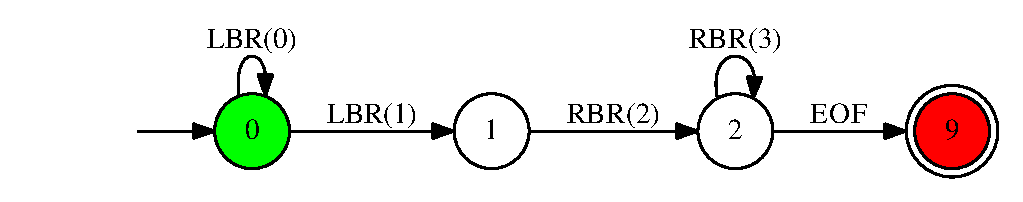
\includegraphics[scale=0.3]{dot/in3.eps}
   }  
   \hfill
    \subfloat[SPPF\label{resultSPPF}]{%
      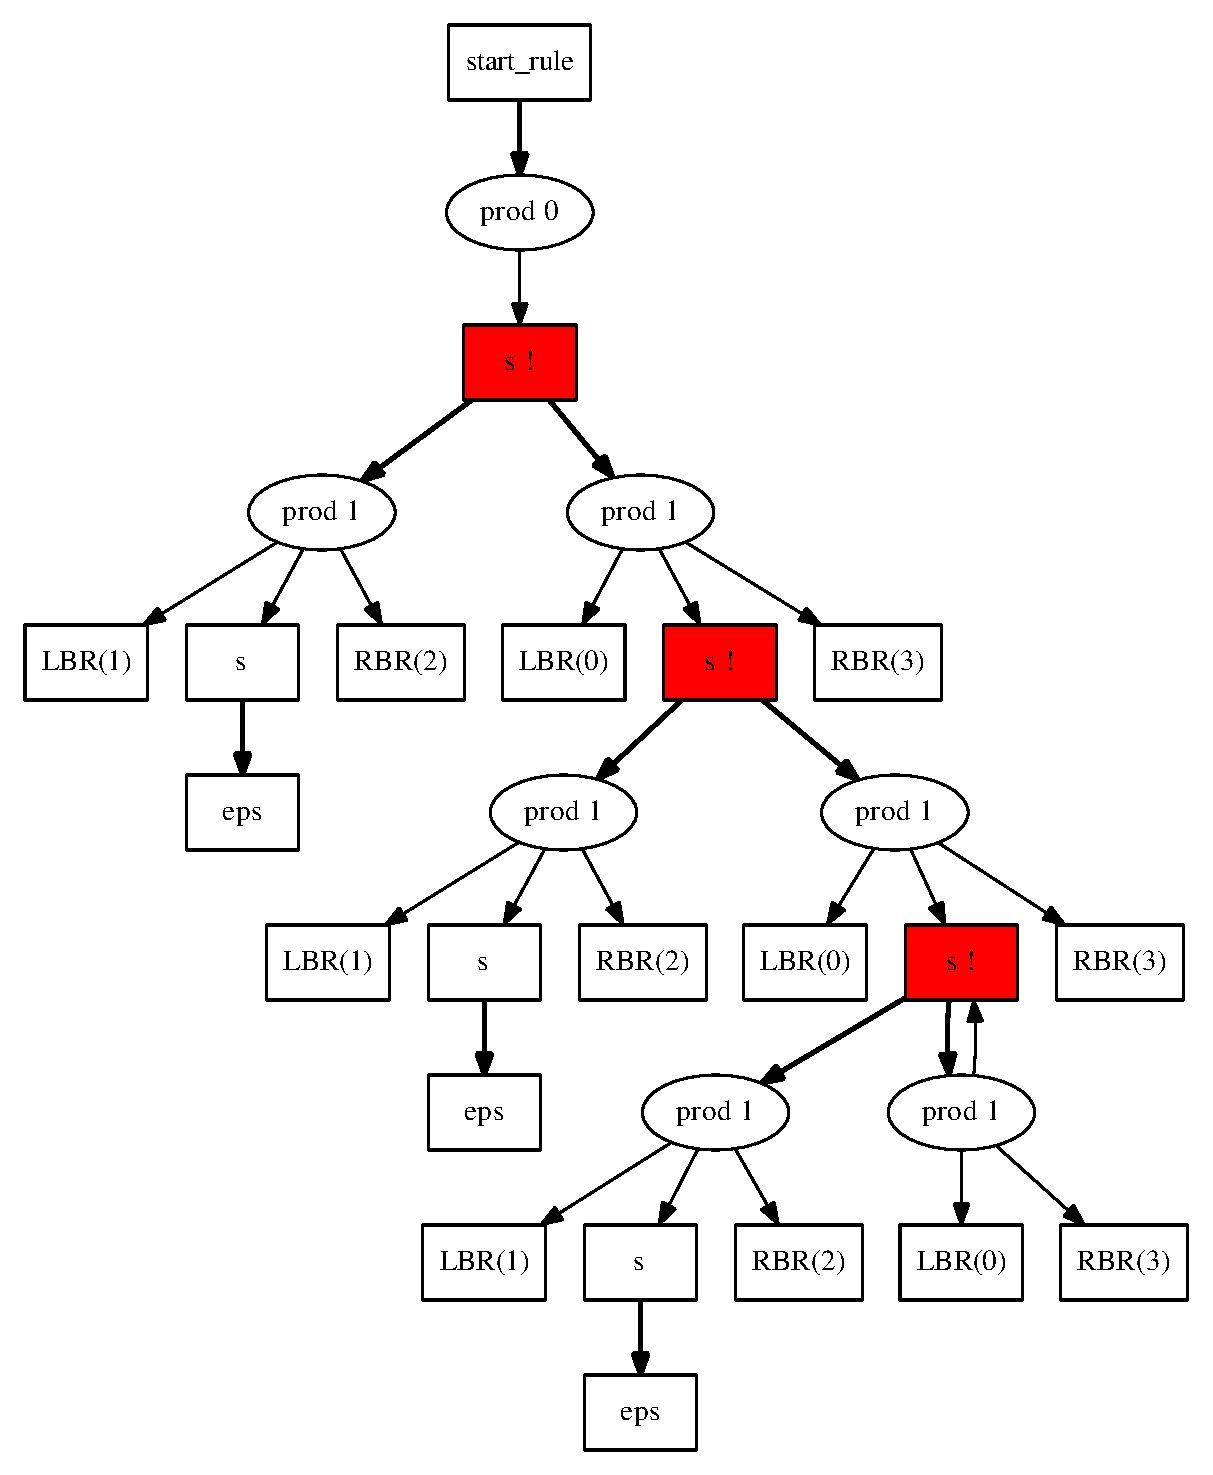
\includegraphics[scale=0.3]{dot/out3.eps}
    }
    \caption{Regular approximation and SPPF}
    \label{fig:SPPFforReg}
 \end{figure}

%\begin{figure}
%    \begin{center}
%        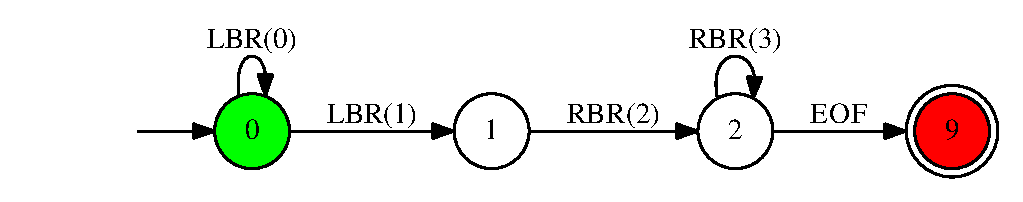
\includegraphics[scale=0.5]{dot/in3.eps}
%    \end{center}
%    \caption{$A_1$ -- input for our algorithm: regular approximation for string-embedded code after tokenization} 
%    \label{faApprox}
%\end{figure}

As it can be seen, some of the words from regular approximation do not belong to the reference language (for example, 
\verb|LBR LBR RBR|). The algorithm ignores such strings and constructs SPPF, which contains derivation trees 
for all recognized strings w.r.t. reference grammar.

%\begin{figure}
%    \begin{center}
%        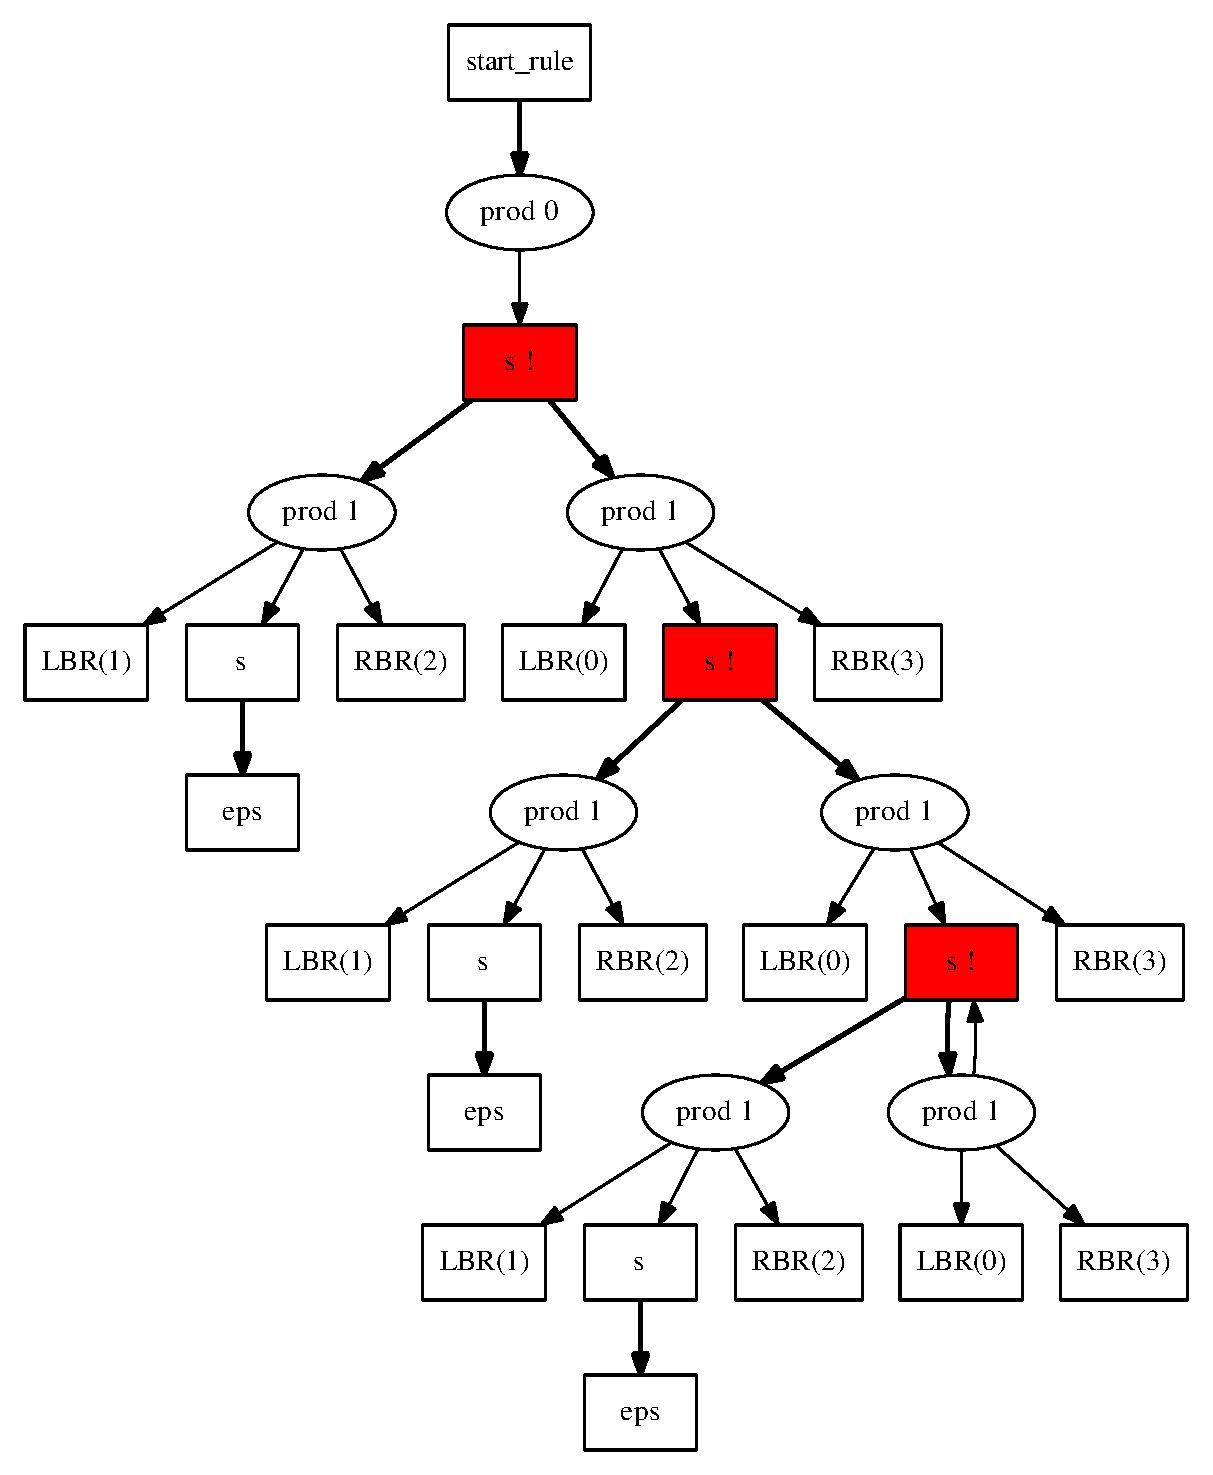
\includegraphics[scale=0.3]{dot/out3.eps}
%    \end{center}
%    \caption{SPPF for input FA presented in figure~\ref{faApprox}}
%    \label{resultSPPF}
%\end{figure}
\pagebreak
\section{\appendixname: RNGLR pseudocode}\label{RNGLRCode}

\begin{algorithm}[]
\begin{algorithmic}[1]
\caption{RNGLR algorithm}
\label{rnglr}
\Function{parse}{$grammar, input$}
  \State{$\mathcal{R} \gets \emptyset$} \Comment{Queue of tuples of GSS vertex, nonterminal, and reduction length}
  \State{$\mathcal{Q} \gets \emptyset$} \Comment{Collection of pairs of GSS vertex and parser state}
  \If{$input = \epsilon$}
    \If{$grammar$ accepts empty input} {report success}
    \Else { report failure}
    \EndIf
  \Else
    \State{\Call{addVertex}{$0, 0, startState$}}
    \ForAll{$i$ in $0..input.Length-1$}
      \State{\Call{reduce}{$i$}}
      \State{\Call{push}{$i$}}
    \EndFor
    \If{$i=input.Length-1$ and there is a vertex in the last level of GSS which state is accepting}
      \State{report success}
    \Else { report failure}
    \EndIf
  \EndIf
\EndFunction
\Function{reduce}{$i$}
  \While{$\mathcal{R}$ is not empty}
    \State{$(v, N, l) \gets \mathcal{R}.Dequeue()$}
    \State{find the set $\mathcal{X}$ of vertices reachable from $v$ along the path of length $(l-1)$}
    \State{or length $0$ if $l=0$}
    \ForAll{$v_{h} = (level_{h}, state_{h})$ in $\mathcal{X}$}
      \State{$state_{t} \gets$ calculate new state by $state_{h}$ and nonterminal $N$}
      \State{\Call{addEdge}{$i, v_{h}, v.level, state_{tail}, (l=0)$}}
    \EndFor
  \EndWhile
\EndFunction
\Function{push}{$i$}
  \State{$\mathcal{Q^{'}} \gets$ copy $\mathcal{Q}$}
  \While{$\mathcal{Q^{'}}$ is not empty}
    \State{$(v, state) \gets \mathcal{Q}.Dequeue()$}
    \State{\Call{addEdge}{$i, v, v.level + 1, state, false$}}
  \EndWhile
\EndFunction
\end{algorithmic}
\end{algorithm}

\begin{algorithm}[]
\begin{algorithmic}[1]
\caption{GSS construction}
\label{RNGLRMain}
\Function{addVertex}{$i, level, state$}
  \If{GSS does not contain vertex $v = (level, state)$}
    \State{add new vertex $v = (level, state)$ to GSS}
    \State{calculate the set of shifts by $v$ and the $input[i+1]$ and add them to $\mathcal{Q}$}
    \State{calculate the set of zero-reductions by $v$ and the $input[i+1]$ and}
    \State{add them to $\mathcal{R}$}
  \EndIf
  \State{\Return{$v$}}
\EndFunction
\Function{addEdge}{$i, v_{h}, level_{t}, state_{t}, isZeroReduction$}
  \State{$v_{t} \gets$ \Call{addVertex}{$i, level_{t}, state_{t}$}}
  \If{GSS does not contain edge from $v_{t}$ to $v_{h}$}
    \State{add new edge from $v_{t}$ to $v_{h}$ to GSS}
    \If{not $isZeroReduction$}
      \State{calculate the set of reductions by $v$ and the $input[i+1]$ and}
      \State{add them to $\mathcal{R}$}
    \EndIf
  \EndIf
\EndFunction
\end{algorithmic}
\end{algorithm}




\end{document}
